\documentclass[a4paper]{article}

\usepackage[english]{babel}
\usepackage[utf8]{inputenc}
\usepackage{amsmath}
\usepackage{amsfonts}
\usepackage{graphicx}
\usepackage[colorinlistoftodos]{todonotes}

\title{Principal Components Analysis}

\author{Cheng Li, Bingyu Wang}

\date{\today}

\begin{document}
\maketitle
\section{What's PCA}

Principal component analysis (PCA) is a statistical procedure that uses an orthogonal transformation to convert a set of observations of possibly correlated variables into a set of values of linearly uncorrelated variables called principal components. The number of principal components is less than or equal to the number of original variables. 

In another word, PCA tries to identify the subspace in which the data approximately lies. Here are two examples given by Andrew Ng's Notes:

	1) Given a dataset \{$x^{(i)}; i = 1, ..., m$ \} of attributes of m different types of automobiles, such as their maximum speed, turn radius, and so on. Let $x^{(i)} \in \mathbb{R}^{n}$ for each $i$. But unknown to us, two different features-some $x_i$ and $x_j$-respectively give a car's maximum speed measured in miles per hour, and maximum speed measured in kilometers per hour. These two features are therefore almost linearly dependent, up to only small differences introduced by rounding off to the nearest $mph$ and $kph$. Thus the data really lies approxmimately on an $n-1$ dimensinal subspace. How can we automatically detect, and perhaps remove, this redundancy?
    
    2) For a less contrived example, consider a dataset resulting from a survey of pilots for radio-controlled helicopters, where $x_1^{i}$ is a measure of the piloting skill of pilot i, and $x_2^{i}$ captures how much he/she enjoys flying. Because RC helicopters are very difficult to fly, only the most committed students, ones that truly enjoy flying, become a good pilots. So, the two features $x_1$ and $x_2$ are strongly correlated. Indeed, we might posit that the data actually likes along some diagonal axis (the $u_1$ direction) capturing the intrinsic piloting "karma" of a person, with small amount of noise lying off this axis. (See Figure\ref{fig:pilot}) How can we automatically compute this $u_1$ direction?
    
\begin{figure}[h]
\centering
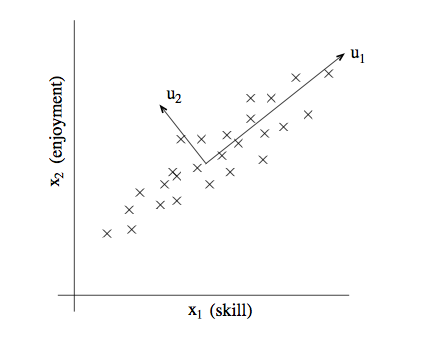
\includegraphics[width=0.7\textwidth]{./images/pilot_example.png}
\caption{\label{fig:pilot} Pilot's skill and enjoyment relationship.}
\end{figure}

\section{Prior PCA algorithm}

Before running PCA, typically we first pre-process the data to normalize its mean and variance, as following:

\begin{enumerate}
\item Let $u = \frac{1}{m} \sum_{i=1}^{m} x^{(i)}$
    \item Replace each $x^{(i)}$ with $x^{(i)} - u$
    \item Let $\sigma_j^2 = \frac{1}{m} \sum_{i=1}^{m} (x_j^{(i)})^2$
    \item Replace each $x_j^{(i)}$ with $\frac{x_j^{(i)}}{\sigma_j}$
\end{enumerate}

Step $1-2$ zero out of the mean of the data, and may be omitted for data known to have zero mean(for instance, time series corresponding to speech or other acoustic signals.) 

Step $3-4$ rescale each coordinate to have unit variance, which ensures that different attributes are all treated on the same "scale". For instance, if $x_1$ was car's maximum speed in $mph$(taking values from \{$10-200$\}) and $x_2$ are the number of seats(taking values from \{$2-8$\}), then this renormalization rescales the different features to make them more comparable. Step $3-4$ may be omitted if we had apriori knowledge that the different features are all on the same scale(for instance, the MNIST digits dataset).


\section{PCA Theory}

After the prior Steps $1-4$, which has been described above, all we have to do is just only an eigenvector calculation. Then we just choose the top $k$ eigenvectors as the new subspace. Why does it work and what is the theory behind the PCA? In fact, there are many theories can explain the PCA. But we just choose one of them, called Maximum Variance theory.

\subsection{Maximum Variance Theory}

Having carried out the normalization, how do we compute the "major axis of variation" $u$-that is, the direction on which the data approximately lies? One way to pose this problem is as finding the unit vector $u$ so that when the data is projected onto the direction corresponding to $u$, the variance of the projected onto the direction corresponding to $u$, the variance of the projected data is maximized. Intuitively, the data starts off with some amount of variance/information in it. We would like to choose a direction $u$ so that if we were to approximate the data as lying in the direction/subspace corresponding to $u$, as much as possible of this variance is still retained.

\subsection{Analysis}

Consider the following dataset(See Figure \ref{fig:sample}), on which we have already carried out the normalization steps:
\begin{figure}[h]
\centering
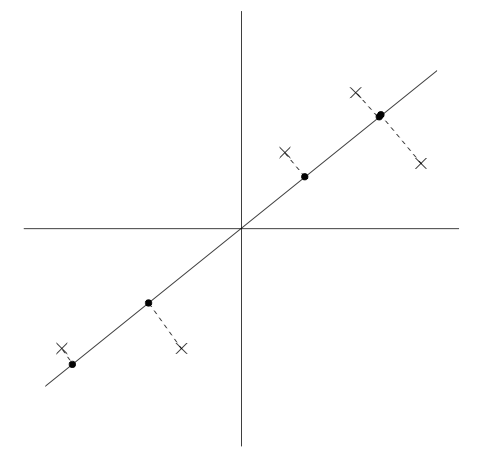
\includegraphics[width=0.7\textwidth]{./images/sample.png}
\caption{\label{fig:sample} Sample data in 2-Dimention}
\end{figure}
Now, suppose we pick $u$ to correspond the direction shown in Figure \ref{fig:samplemax}. The circles denotes the projections of the original data onto this line.
\begin{figure}[h]
\centering
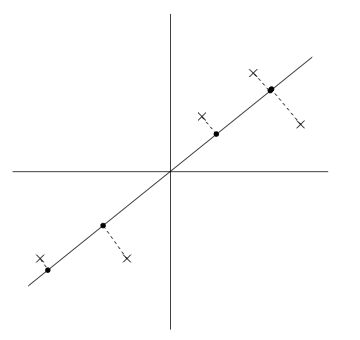
\includegraphics[width=0.7\textwidth]{./images/sample_max.png}
\caption{\label{fig:samplemax} Sample data with Maximum Variance}
\end{figure}
\begin{figure}[h]
\centering
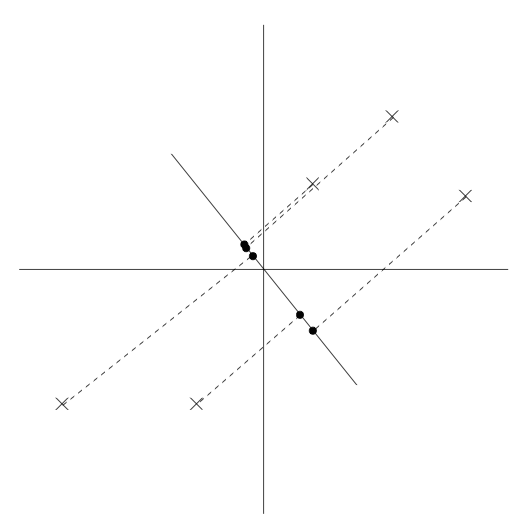
\includegraphics[width=0.7\textwidth]{./images/sample_min.png}
\caption{\label{fig:samplemin} Sample data with Minimum Variance}
\end{figure}

We see that in Figure \ref{fig:samplemax} the projected data still has a fairly large variance, and the points tend to be far from zero. In contrast, suppose had instead picked the following direction(Figure \ref{fig:samplemin}):

In the Figure \ref{fig:samplemin}, the projections have a significantly smaller variance, and are much closer to the origin.

We would like to automatically select the direction $u$ corresponding to the Figure \ref{fig:samplemax} with maximum variance.  First we should know how to calculate the distance of the point's projection onto $u$ from the origin. Note that given a unit vector $u$ and a point $x$, the length of the projection of $x$ onto $u$ is given by $x^{T}u$. So the problem can be transformed to mathematic problem as following: choose $u$ so that:
$$
	\max_{u:\begin{Vmatrix}u\end{Vmatrix}=1} \frac{1}{m} \sum_{i=1}^{m}(x^{(i)T}u)^{2}
$$

Next, we will derivate the fomular as following:
\begin{align*}
	&\implies \max_{u:\begin{Vmatrix}u\end{Vmatrix}=1} \frac{1}{m} \sum_{i=1}^{m}(x^{(i)T}u)^{2} \\ 
	&\implies \max_{u:\begin{Vmatrix}u\end{Vmatrix}=1} \frac{1}{m} \sum_{i=1}^{m}(x^{(i)T}u)^{T}(x^{(i)T}u) \\
	&\implies \max_{u:\begin{Vmatrix}u\end{Vmatrix}=1} \frac{1}{m} \sum_{i=1}^{m}(u^Tx^{(i)})(x^{(i)T}u) \\
	&\implies \max_{u:\begin{Vmatrix}u\end{Vmatrix}=1} \frac{1}{m} \sum_{i=1}^{m}u^Tx^{(i)}x^{(i)T}u \\ 
	&\implies \max_{u:\begin{Vmatrix}u\end{Vmatrix}=1} u^T (\frac{1}{m}\sum_{i=1}^{m}x^{(i)}x^{(i)T})u \\
	&\implies \max_{u:\begin{Vmatrix}u\end{Vmatrix}=1} u^T \Sigma u, \quad where \quad \Sigma=\frac{1}{m}\sum_{i=1}^{m}x^{(i)}x^{(i)T}
\end{align*}

Now we can use Lagrange multiplier to continue: 
\begin{align*}
	&\implies \max u^T \Sigma u \quad \quad subject\quad u^Tu = 1(Because \begin{Vmatrix}u\end{Vmatrix}=1) \\
	&\implies \mathcal{L}(u,\lambda) = u^T \Sigma u + \lambda (u^Tu - 1) \\
	&\implies \frac{\partial \mathcal{L}(u,\lambda)}{\partial u} = \frac{\partial(u^T\Sigma u+\lambda u^Tu)}{\partial u}
    = \Sigma u - \lambda u \overset{Set}{=} 0 \\
	&\implies \Sigma u = \lambda u
\end{align*}

Finally, we get the $\Sigma u = \lambda u$, where $u$ is the engivector of $\Sigma$ and $\lambda$ is the engivalue of  $\Sigma$.

To summarize, we have found that if we wish to find a 1-dimensional subspace with to approximate the data, we should choose $u$ to be the principal eigenvector of $\Sigma$. More generally, if we wish to project our data to k-dimensional subspace ($k<n$), we should choose $u_1, u_2, ..., u_k$ to be the top $k$ vectors of $\Sigma$. The $u_i$'s now form a new, orthogonal basis for the data.\footnote{Because $\Sigma$ is symmetric, the $u_i$'s will (or always can be chosen to be) orthogonal to each other.}

Then, to represent $x^{(i)}$ in this basis, we need only compute the corresponding vector
$$
	y^{(i)} = \begin{bmatrix} 
	u_1^Tx^{(i)} \\
	u_2^Tx^{(i)} \\
	... \\
	u_k^Tx^{(i)} \end{bmatrix}
	\in \mathbb{R}^{k}.
$$
Thus, whereas $x^{(i)} \in \mathbb{R}^n$, the vector $y^{(i)}$ now gives a lower, k-dimensional, approximation/representation for $x^{(i)}$. PCA is therefore also referred to as a \textbf{dimensionality reduction} algorithm. The vectors $u_1, ..., u_k$ are called the first k \textbf{principal components} of the data.

\section{References}

\begin{itemize}
    \item PCA Lecture Notes by Andrew Ng(Stanford Univ.).    
\end{itemize}
\end{document}